%
% This document is licensed under the
%
%   Creative Commons Attribution-Noncommercial-Share Alike
%
% license. Please see LICENSE file for details.
%

\documentclass{InsightArticle}

\usepackage[dvipdfm]{graphicx}
\usepackage{url}

\usepackage[dvipdfm,
bookmarks,
bookmarksopen,
backref,
colorlinks,linkcolor={blue},citecolor={blue},urlcolor={blue},
]{hyperref}


\title{User Guide to \\[4mm] The Computational Morphometry
  Toolkit\footnote{This document is licensed under
    the Creative Commons Attribution License Version 3.0.}}

\release{1.10}

\author{Torsten Rohlfing}
\authoraddress{Neuroscience Program, SRI International, Menlo Park, CA\footnote{Continued development and maintenance of CMTK is funded by
    the NIBIB under Grant No. R01~EB008381.}}

\begin{document}

\maketitle

\ifhtml
\chapter*{Front Matter\label{front}}
\fi


\begin{abstract}
\noindent This guide is intended as a very brief introduction of the main
tools in the Computational Morphometry Toolkit (CMTK), which is available in
source code and as pre-compiled binaries from
http://www.nitrc.org/projects/cmtk/. The target audience of this document are
CMTK users, who might use this document as a reference to the most common
processing tasks, and prospective users, who may find this information useful
to determine whether CMTK provides functionality that they can use. We focus
in particular on a simplified workflow for deformation morphometry studies
based on magnetic resonance images: DICOM conversion, artifact correction,
affine and nonlinear image registration, reformatting, Jacobian determinant
map generation, and statistical hypothesis testing.
\end{abstract}

\clearpage
\tableofcontents

\clearpage
\section{Introduction}

The Computational Morphometry Toolkit, or short CMTK, is a set of software
tools that perform various types of processing and analysis on
three-dimensional (3D) image data. CMTK is available both in source code
(licensed under the GNU GPL3) and as pre-compiled binaries from
\url{http://www.nitrc.org/projects/cmtk/}.

CMTK is primarily a collection of command line tools, which make the toolkit
ideally suited for unattended batch processing of large amounts of data. In
addition, CMTK's back-end libraries, which are shared by all command line
tools, can be used as a relatively lightweight, yet powerful, platform for
implementation of new image processing algorithms.

\LaTeX\ source for this User Guide, including all figures, can be checked out
from the CMTK Subversion repository via
\begin{verbatim}
svn co https://nitrc.org/svn/cmtk/trunk/doc/UserGuideCMTK/
\end{verbatim}

\subsection{Coordinate Conventions}

For medical image data, CMTK uses an anatomy-based coordinate system, which we
refer to as ``RAS'' coordinates. This means that the $x$ direction of the
coordinate space increases towards the anatomical ``Right,'' the $y$ direction
increases towards the anatomical ``Anterior,'' and the $z$ direction increases
towards the anatomical ``Superior.'' The coordinate space origin, $(0,0,0)$,
thus coincides with the ``Left-Posterior-Inferior'' corner of the image
volume. 

All images that are read into one of CMTK's tools are first reoriented to fit
this coordinate system. This means that the storage order of image pixels in
memory is such that the fastest-varying of the three pixel indexes corresponds
to the ``Left''--''Right'' anatomical direction, the second fastest to the
``Posterior''--''Anterior'' direction, and the slowest varying to the
``Inferior''--''Superior'' direction. Consequently, the first pixel in memory
is the one that is the Left-Posterior-Inferior-most pixel anatomically.

For image file formats that define subject orientation based on direction
vectors within an anatomy-based coordinate space, which is the majority of
modern formats, CMTK determines the nearest anatomical orientation of the
image within $\pm 45$ degrees around each rotation axis.

To confirm that images are read correctly, and to diagnose problems, CMTK
comes with a very simple triplanar image viewer (see screen shot in
Fig.~\ref{fig:triplanar}), adequately named ``\verb|triplanar|.'' The
coordinates shown in this viewer for any image are exactly the coordinates
that all CMTK tools use. Note that for the triplanar viewer to be available,
CMTK must be built with support for the Qt
toolkit\footnote{\url{http://qt.nokia.com}} (version 4.3.0 or higher), and the
``\verb|BUILD_GUI|'' build option must be enabled.

\begin{figure}[tbp]
\centerline{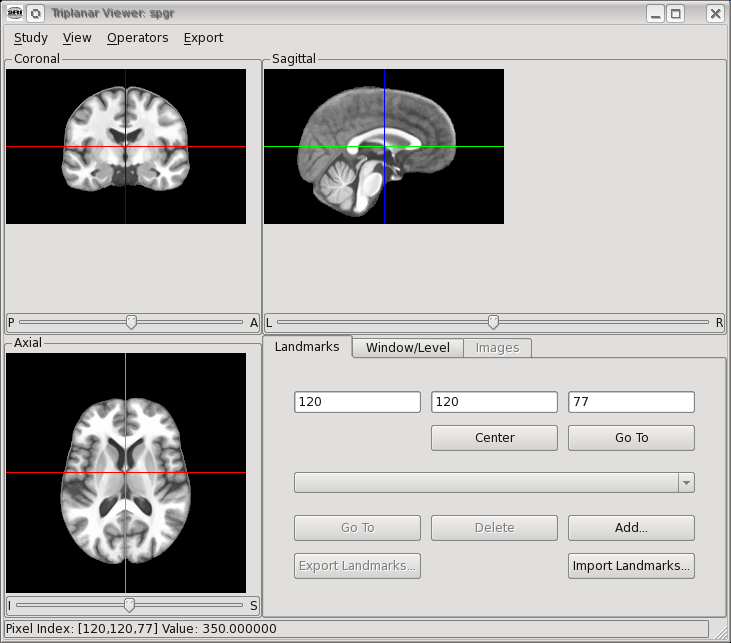
\includegraphics[width=.5\linewidth]{img/triplanar}}
\caption{Screen shot of CMTK's triplanar image viewer.}
\label{fig:triplanar}
\end{figure}

\subsection{Registration Terminology}

Since one of the primary strengths of CMTK is its selection of powerful and
well-tested registration tools, we shall first clarify some important
registration terminology. In pairwise registration, throughout this guide as
well as in all tools and source code, we shall refer to one image as the
reference and the other as the floating image. Others may refer to these as
the fixed and the moving image, respectively. By definition, all coordinate
transformations computed by CMTK are functions that map {\em from\/} the space
of the reference (fixed) image {\em to\/} the space of the floating (moving)
image. As a result, when reformatting one image to match the other, it is the
floating image by default that will be transformed to match the reference
image.

Note that when we speak about transforming coordinates of features, such as
landmarks or the nodes in a mesh, then the coordinates of the reference image
will be transformed to match the floating image.

\subsection{Supported Image File Formats}

CMTK supports a wide range of image file formats, both for import and
export. When reading an image file into CMTK, its type is detected
automatically. Note that in order to correctly identify the format of images
with separate header and data files, it is necessary to provide CMTK with the
path to the header file, not the data file.

Whether a particular file can be read into CMTK can easily be tested using
CMTK's \verb|describe| tool. For example, to test (and describe) the content
of an Analyze 7.5\footnote{\url{http://eeg.sourceforge.net/ANALYZE75.pdf}}
header/image pair, \verb|example.hdr| and \verb|example.img|, one would run
the following command:
\begin{verbatim}
describe example.hdr
\end{verbatim}

When writing files, CMTK determines the desired file format based on the
suffix of the output path. The following suffixes are supported:
\begin{description}
\item [nii] Single-file NIfTI-1 image\footnote{\url{http://nifti.nimh.nih.gov/nifti-1/}}.
\item [img] NIfTI image with detached header. Header file will be written with
  suffix \verb|.hdr|
\item [nrrd] Single-file Nrrd\footnote{\url{http://teem.sourceforge.net/nrrd/}}.
\item [nhdr] Nrrd with detached header. The data file will be written with
  \verb|.raw| suffix.
\item [hdr] Analyze 7.5 detached header. The data file will be written with
  suffix \verb|img|.
\end{description}

{\bf Note} that both Analyze and NIfTI header/data file pairs use the suffixes
\verb|.hdr| and \verb|.img|. For historic reasons, using \verb|.hdr| as the
output file suffix will always invoke Analyze export, whereas the \verb|.img|
suffix will invoke NIfTI export. Both formats need to be read using the
\verb|.hdr| file, however.

{\bf Note} also that, by default, all data files are written with \verb|gzip|
compression. Because CMTK contains a bundled \verb|zlib| library, this is true
even when the \verb|gzip| tool itself is not installed. This behavior can be
disabled by defining the \verb|CMTK_WRITE_UNCOMPRESSED| environment
variable. On a Unix/Linux system using the \verb|csh| shell, this would be
achieved via
\begin{verbatim}
export CMTK_WRITE_UNCOMPRESSED=1
\end{verbatim}
where only the definition of the variable is relevant, and its value is
ignored. Thus, to re-enable compressed writing, rather than setting the
variable to ``0'' for example, use
\begin{verbatim}
unset CMTK_WRITE_UNCOMPRESSED
\end{verbatim}
or its appropriate equivalent inside your favorite shell.

\clearpage
\section{Step-by-Step Morphometry}

This section provides a step-by-step guide to the tools used in a typical
morphometry study using the CMTK tools. It is not intended to provide a
complete list of available tools. We are also not covering all available
options of each tool. Note that a complete list of supported options can
always be obtained by running a given tool with the \verb|--help| command line
option.

\subsection{DICOM Image Stacker}

When dealing with 3D medical image data in particular, the first step of
processing is usually the conversion of a stack of single-slice image files in
DICOM format to a single-file 3D image. To this end, CMTK provides a tool that
can search through a file system tree, find all DICOM files in it, group the
ones that form 3D image volumes, and write each of these volumes into a
separate file in one of the supported formats.

For example, the command
\begin{verbatim}
dcm2image --recurse --out-pattern image%N.nii /path/to/dicom
\end{verbatim}
or short
\begin{verbatim}
dcm2image -r -O image%N.nii /path/to/dicom
\end{verbatim}
would recursively search the file system under {\tt /path/to/dicom} and write
all resulting image volumes to consecutively numbered image files in NIfTI
format, {\tt image-1.nii},  {\tt image-2.nii}, and so on.

\subsection{Interleaved Image Motion Artifact Correction}

\begin{figure}[tbp]
\begin{center}
\begin{tabular}{cc}
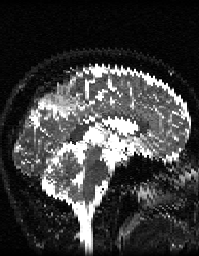
\includegraphics[width=.3\linewidth]{img/film_artifacts}&
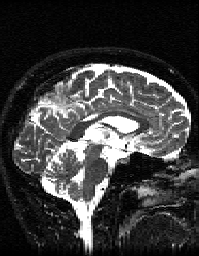
\includegraphics[width=.3\linewidth]{img/film_corrected}
\end{tabular}
\end{center}
\caption{Example of interleaved image before (left) and after (right)
  correction of motion artifacts using the {\tt film} tool. These are roughly
  mid-sagittal slices through a late-echo FSE image acquired in three
  interleaved passes.}
\label{fig:InterleavedExample}
\end{figure}

When MR images are acquired as multiple interleaved sparse image stacks
(``passes''), subject motion between the passes can lead to characteristic
artifacts in the final, interleaved image stack (see
Fig.~\ref{fig:InterleavedExample} for an example). CMTK implements an
algorithm for post-reconstruction correction of these
artifacts~\cite{RohlRadePfef:2008a} in the \verb|film| tool (for ``Fix
InterLeaved Motion'').

The \verb|film| tool operates in three stages: first, the interleaved image
stack is separated into the original passes, and all passes are co-registered
using rigid intensity-based registration to determine the inter-pass motion
parameters. Second, volume injection is used to obtain a coarse reconstructed,
motion-corrected image, which is then refined in the third stage using an
iterative inverse interpolation algorithm (see Ref.~\cite{RohlRadePfef:2008a}
for details).

For proper operation, the \verb|film| tool needs to be given the number of
passes in the interleaved images, for example for a three-pass image:
\begin{verbatim}
film --passes 3 input.nii corrected.nii
\end{verbatim}
In most cases, the through-plane acquisition direction can be guessed from the
data.

\subsection{MR Intensity Bias Field Correction}

CMTK implements a model-free algorithm for intensity bias field correction
based on minimization of image entropy~\cite{LikaVierPern:2001}. The
\verb|mrbias| tool, which implements this algorithm, is typically called as
follows:
\begin{verbatim}
mrbias --degree-mul 2 --mask foreground.nii spgr.nii spgr_corrected.nii
\end{verbatim}
which computes a second-order polynomial multiplicative bias
field. Computation is constrained via a (binary) mask that is read from the
\verb|foreground.nii| image. Alternatively, the tool can generate its own mask
via the \verb|--thresh-min| and  \verb|--thresh-max| command line parameters.

\begin{figure}[tbp]
\begin{center}
\begin{tabular}{cc}
Original & Corrected \\
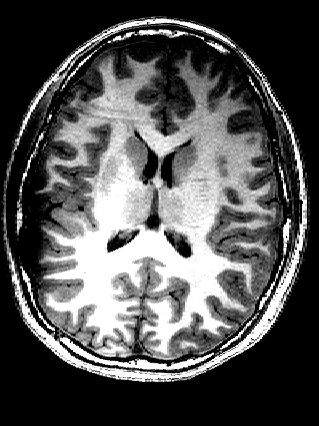
\includegraphics[width=.3\linewidth]{img/mrbias_orig}&
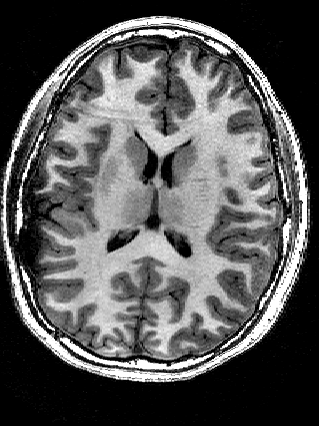
\includegraphics[width=.3\linewidth]{img/mrbias_corr} \\
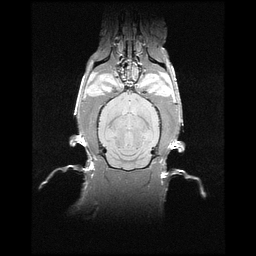
\includegraphics[width=.3\linewidth]{img/mrbias_rat_early_orig}&
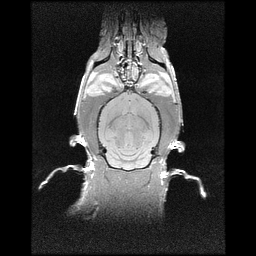
\includegraphics[width=.3\linewidth]{img/mrbias_rat_early_corr}
\end{tabular}
\end{center}
\caption{Examples of MR intensity bias field correction using a second-order
polynomial multiplicative bias field computed by the {\tt mrbias} tool. {\em
  Top row:\/} applied to a human brain SPGR image acquired at 3T.  {\em
  Bottom row:\/} applied to a rat brain early-echo FSE image acquired at 3T.}
\label{fig:Mrbias}
\end{figure}

One of the advantages of this particular algorithm for intensity bias field
correction is that it does not involve a model of either the anatomy in the
image or the tissue types that are present. It, therefore, works well on human
as well as non-human images (Fig.~\ref{fig:Mrbias}), and on brain as well as
non-brain anatomy, such as abdominal images.

To generate foreground masks automatically, CMTK provides a very simple
``levelset-type'' segmentation tool:
\begin{verbatim}
levelset --binarize spgr.nii foreground.nii
\end{verbatim}
In very broad terms, the tool implements an extreme simplification of the
algorithm for segmentation without edges by Chan \&
Vese~\cite{ChanVese:2001}. By default, the tool writes an image that is the
resulting levelset function, but using the \verb|--binarize| switch turns the
output into a thresholded, binary mask that is appropriate for use by the
\verb|mrbias| tool.

\begin{figure}[tb]
\begin{center}
\begin{tabular}{ccc}
Image & Mask & Image with Mask Outline \\
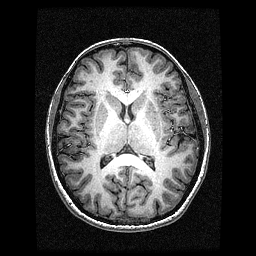
\includegraphics[width=.3\linewidth]{img/levelset_spgr_spgr}&
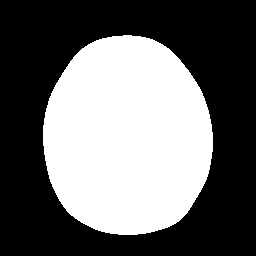
\includegraphics[width=.3\linewidth]{img/levelset_spgr_mask}&
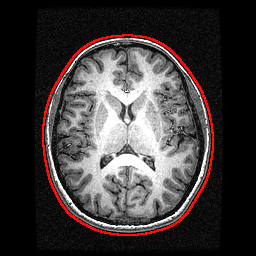
\includegraphics[width=.3\linewidth]{img/levelset_spgr_ovl} \\
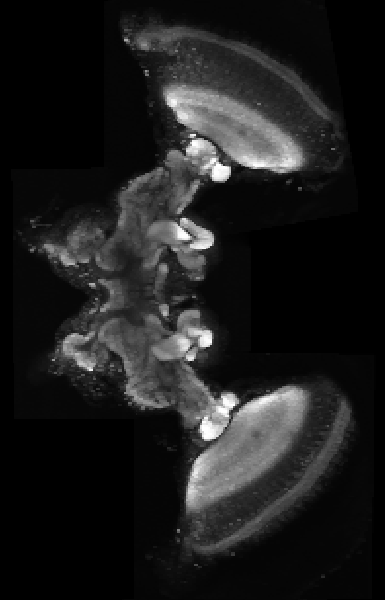
\includegraphics[width=.3\linewidth]{img/levelset_locust_clsm}&
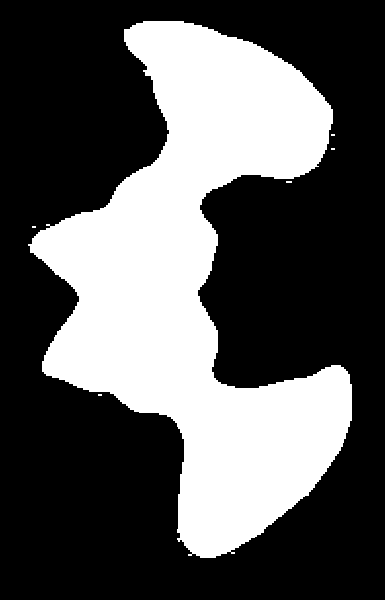
\includegraphics[width=.3\linewidth]{img/levelset_locust_mask}&
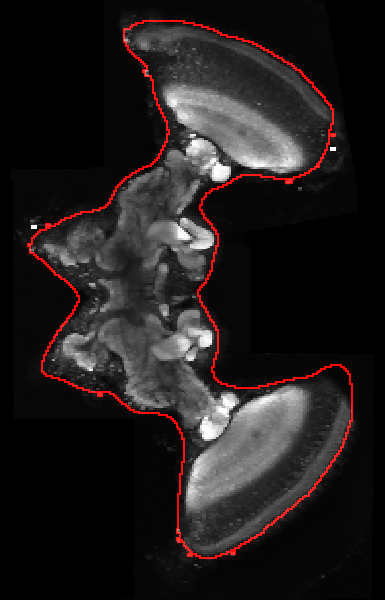
\includegraphics[width=.3\linewidth]{img/levelset_locust_ovl}
\end{tabular}
\end{center}
\caption{Examples of foreground/background segmentation using the {\tt
levelset} tool. {\em Top row:\/} SPGR image acquired at 3T. {\em Bottom
row:\/} fluorescent confocal laser scanning microscopy image of a locust
brain~\cite{KuryRohlKrof:2008}. Both examples were computed by running the
{\tt levelset} tool with default settings and no image-specific
parameters. [Locust images courtesy of U.~Homberg, Universit\"at Marburg
(Germany).]  }
\label{fig:Levelset}
\end{figure}

\subsection{Affine Image Registration}

The basic pairwise image registration tool in CMTK, \verb|registration|,
implements an algorithm similar to the multi-resolution algorithm by Studholme
{\em et al.\/}~\cite{StudHillHawk:1997}. More technical detail about our
implementation in particular can be found in Ref.~\cite{Rohlfing:2000}, albeit
only in German.

In order to compute an affine registration between two images, the
registration tool can be run as follows:
\begin{verbatim}
registration --initxlate --dofs 6,9 --auto-multi-level 4 \
        -o affine.xform ref.nii flt.nii
\end{verbatim}
This performs a registration of the floating image, \verb|flt.nii|, to the
reference image, \verb|ref.nii|, where all optimization and image resampling
parameters are automatically determined for a 4-level multi-resolution
procedure. 

At each resolution level, the registration first optimizes 6 degrees of
freedom (DOF), i.e., translation and rotation of a 3D rigid
transformation. Afterwards, 9 DOFs are optimized, i.e., three anisotropic
scale factors in addition to the translational and rotational
parameters. Supported DOF numbers are: 0 (no registration, for testing),
3 (translation only), 6 (rigid: translation, rotation),  7 (similarity:
translation, rotation, global scale), 9 (translation, rotation, anisotropic
scale), and 12 (full affine: translation, rotation, scale, and shears).

By default, registration uses the normalized mutual
information~\cite{StudHillHawk:1999} image similarity measure. Other available
similarity measures are: standard mutual
information~\cite{MaesCollVand:1997,WellViolAtsu:1996} (\verb|--mi|), mean
squared difference (\verb|--msd|), normalized cross-correlation
(\verb|--ncc|), and correlation ratio~\cite{RochMalaPenn:1998a} (\verb|--cr|)

In the above example, the registration transformation is initialized (via
\verb|--initxlate|) by translating the floating image's center to that of the
reference image. For more complex initializations, the
\verb|make_initial_affine| tool can be used, which supports centers of mass,
principal axes~\cite{AlpeBradKenn:1990}, and image orientation vectors (e.g.,
as provided by the original DICOM data).

For example, in order to first initialize a transformation using principal
axes and then use the result as the initial transformation for intensity-based
refinement, one would use the following sequence of commands:
\begin{verbatim}
make_initial_xform --principal-axes ref.nii flt.nii initial.xform
registration --initial initial.xform --dofs 6,9 --auto-multi-level 4 \
        -o affine.xform ref.nii flt.nii
\end{verbatim}

\subsection{Nonrigid Image Registration}

Pairwise nonrigid image registration in CMTK implements an algorithm
introduced by Rueckert {\em et al.\/}~\cite{RuecSonoHaye:1999}, which uses
as its transformation model multi-resolution free-form deformations based on
cubic spline interpolation between sparse, uniformly distributed control
points. Our particular implementation, which uses SMP parallelism to take
advantage of multi-CPU systems, was described in Ref.~\cite{RohlMaur:2003}.

A very simple nonrigid registration using a 40\,mm control point grid,
registering floating image \verb|flt.nii| to reference image \verb|ref.nii|
based on an affine transformation \verb|affine.xform| can be run as follows:
\begin{verbatim}
warp -o ffd40.xform --grid-spacing 40 --initial affine.xform ref.nii flt.nii
\end{verbatim}
Typically, however, one would want to run a more sophisticated multi-level
deformation, say with three refinements (each reducing the grid spacing by
1/2 for a final spacing of 5\,mm), and constrain the deformation using grid
bending energy:
\begin{verbatim}
warp -o ffd5.xform --grid-spacing 40 --refine 3 --energy-weight 1e-1 \
        --initial affine.xform ref.nii flt.nii
\end{verbatim}
To prevent folding of the deformation grid, it is possible to instead
constrain the Jacobian determinant of the deformation to be nonzero, which is
achieved by changing the above command as follows:
\begin{verbatim}
warp -o ffd5.xform --grid-spacing 40 --refine 3 --jacobian-weight 1e-5 \
        --initial affine.xform ref.nii flt.nii
\end{verbatim}

\subsection{Reformating Registered Images}

To reformat the registered floating image following the examples in
the previous section, run
\begin{verbatim}
reformatx  -o reformat.nii --floating flt.nii ref.nii ffd5.xform
\end{verbatim}
The somewhat unintuitive order of arguments on the command line is due to the
versatility of the \verb|reformatx| tool, which allows for the concatenation
of arbitrary transformations (and their inverses), such as
\begin{verbatim}
reformatx  -o reformat.nii --floating img3.nii \
        img1.nii img1_to_2.xform --inverse img3_to_2.xform
\end{verbatim} 
By default, \verb|reformatx| uses trilinear interpolation, but it also
supports cubic ({\tt --cubic}) and cosine-windowed sinc
({\tt --sinc-cosine}) interpolation for intensity images, partial volume
interpolation~\cite{MaesCollVand:1997} ({\tt --pv}) for label images, and
nearest neighbor ({\tt --nn}) interpolation for all types of images.

\subsection{Jacobian Determinant Maps}

Jacobian determinant maps, which are a staple ingredient of deformation-based
morphometry studies~\cite{AshbHuttFrac:1998}, can also be computed using the
\verb|reformatx| tool. In the simplest case, we may want to compute the
Jacobian determinant map for a transformation \verb|time1_to_time2.xform|
between two images, say images \verb|time1.nii| and \verb|time1.nii| acquired
from the same subject at two time points. The command to compute the
appropriate Jacobian determinant map, \verb|jacobian.nii|, is then
\begin{verbatim}
reformatx  -o jacobian.nii time1.nii --jacobian time1_to_time2.xform
\end{verbatim}
More interestingly, say we want to compare these Jacobian maps from multiple
subjects, all in the space of a common atlas coordinate system. Then, instead
of computing each map first in each subject's coordinate system and then
reformatting these maps into atlas space, we can directly compute the maps in
atlas space by concatenation of transformations:
\begin{verbatim}
reformatx  -o jacobian.nii atlas.nii \
        atlas_to_time1.xform --jacobian time1_to_time2.xform
\end{verbatim}
Here, every sample coordinate in atlas space is first mapped to subject time 1
space via \verb|atlas_to_time1.xform|. For the resulting location, the
Jacobian determinant of the longitudinal transformation,
\verb|time1_to_time2.xform|, is then computed.

Because the nonrigid transformations computed by the \verb|warp| tool are
generated via continuously differentiable B-spline basis functions, we can
compute the Jacobian analytically at any location in the domain of the
transformation, which means that the direct computation of Jacobians into
atlas space does indeed avoid one interpolation of the Jacobian determinant
map.

{\bf Note} that the \verb|reformatx| tool allows an arbitrary number of
transformations to be listed both before and after the \verb|--jacobian|
switch, and any transformation can additionally be inverted by prefixing it
with \verb|--inverse| (affine transformations are inverted explicitly, whereas
nonrigid transformations are inverted numerically). 

\subsection{Statistical Testing}

For group comparisons of, for example, Jacobian determinant maps between
different subject groups, the \verb|ttest| tool computes different types of
t-tests (all two-tailed) and statistics. In the simplest case, two populations
A and B of maps can be tested against one another as follows:
\begin{verbatim}
ttest -o pvalues.nii --tstats-file tstats.nii \
        jacobianA1.nii jacobianA2.nii -- jacobianB1.nii jacobianB2.nii
\end{verbatim} 
This computes a pixel-wise two-tailed {\em unpaired\/} t-test between the two
lists of images separated with ``\verb|--|'' on the command line. The
resulting $p$-values image is then written to \verb|pvalues.nii|, and the
t-statistics are also written to \verb|tstats.nii|.

To compute a two-tailed {\em paired\/} t-test, make sure that there are an
equal number of images before and after the ``\verb|--|'' separator and that
corresponding images in both groups are in the same order, then add the
\verb|--paired| option and run
\begin{verbatim}
ttest -o pvalues.nii --tstats-file tstats.nii --paired \
        jacobianA1.nii jacobianA2.nii -- jacobianB1.nii jacobianB2.nii
\end{verbatim}
Invoking \verb|ttest| with only a single group of images (without
``\verb|--|'' anywhere in the image list), will compute a single-sample
t-test, that is, a test for significant differences from zero:
\begin{verbatim}
ttest -o pvalues.nii --tstats-file tstats.nii jacobianA1.nii jacobianA2.nii
\end{verbatim} 

\subsection{General Linear Modeling}

\cite{FrisHolmWors:1995}

\subsection{Atlas-based Segmentation}

Atlas-based segmentation uses correspondence between a previously segmented
image (the atlas) and a new, unsegmented image to create a segmentation of the
latter~\cite{MillChriAmit:1993}. This relatively simple idea can easily be
implemented using CMTK's \verb|registration|, \verb|warp|, and
\verb|reformatx| tools. For convenience, however, CMTK also provides an
integrated atlas-based segmentation tool, which can be run as follows:
\begin{verbatim}
asegment input_image.nii atlas_image.nii atlas_labels.nii output_labels.nii
\end{verbatim}
Here, it is assumed that \verb|input_image.nii| is a new, unsegmented image,
for example an MR scan of a new subject, \verb|atlas_image.nii| is the
intensity image of the atlas, and \verb|atlas_labels.nii| is the label image
of the atlas, i.e., the segmentation corresponding to the atlas intensity
image. The tool will then register the atlas to the new image, reformat that
atlas label map onto it, and write the result to the file
\verb|output_labels.nii|.

The standard atlas of CMTK is the SRI24
atlas~\cite{RohlZahrSull:2008,RohlZahrSull:2010}, which comprises several
different channels of MR image information, as well as scalar diffusion
measures, tissue probability maps, and segmentation maps. If CMTK is
configured and built with SRI24 support (by setting the
\verb|CMTK_ROOT_PATH_SRI24| CMake variable), then a simplified segmentation
tool, \verb|asegment_sri24|, which uses the SRI24 atlas is also built.

This tool, by default, registers a given image to the SPGR channel of the
SRI24 atlas. It then creates and writes a segmentation map based on the
``tzo116plus'' label map, which derived from the ``automatic anatomic
labelling'' (AAL) parcellation map by Tzourio-Mazoyer {\em et
al.\/}~\cite{TzouLandPapa:2002}. This is achieved simply by running
\begin{verbatim}
asegment_sri24 input_image.nii output_segmentation.nii
\end{verbatim} 
Different atlas channels can be used for registration, selected
using the \verb|--registration-channel| command line option: ``\verb|spgr|''
for T1-weighted SPGR, which is the default,``\verb|early-fse|'' for early-echo
(proton density-weighted) FSE , ``\verb|late-fse|'' for late-echo
(T2-weighted) FSE, and ``\verb|fa|'' for DTI-derived fractional anisotropy.

Likewise, different label maps are available for the output, selected by the
\verb|--label-map| command line option: ``\verb|tzo116plus|'' for the extended
Tzourio-Mazoyer map, ``\verb|lpba40|'' for a segmentation based on the
40-subject LONI Probabilistic Brain Atlas~\cite{ShatMirzAdis:2008}, and
``\verb|tissue|'' for a maximum-likelihood three-tissue (CSF, WM, GM)
segmentation.

\begin{figure}[tb]
\centerline{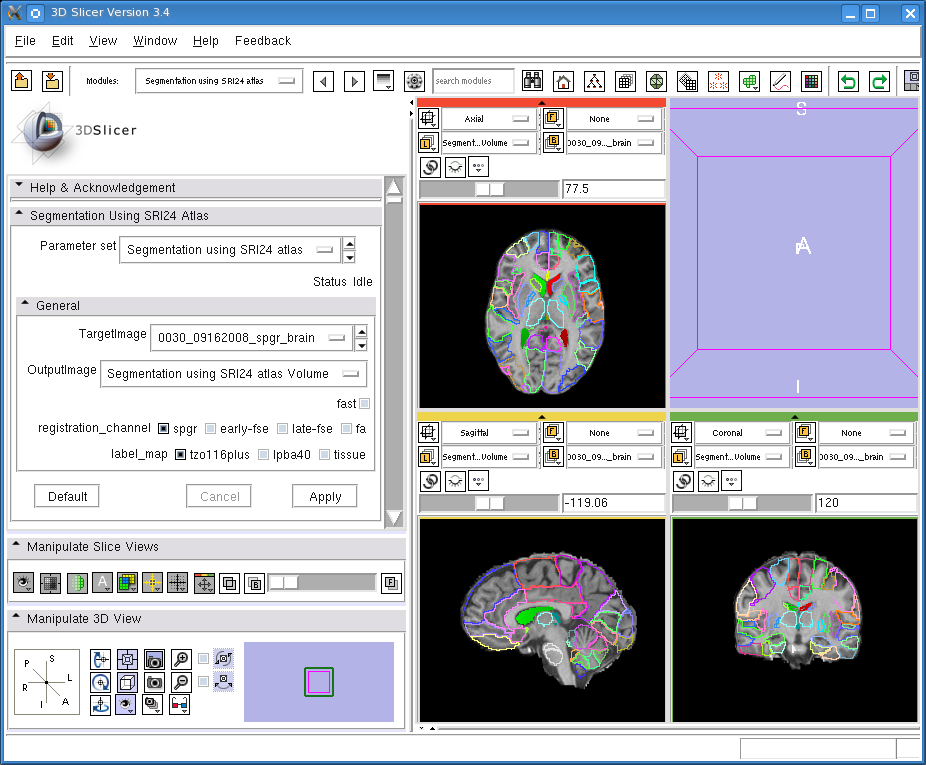
\includegraphics[width=\linewidth]{img/slicer-asegment_sri24}}
\caption{Integration of {\tt asegment\_sri24} tool into 3D Slicer, and result
  of segmentation using the ``{\tt tzo116plus}'' label map.}
\label{fig:SlicerSRI24}
\end{figure}

The integration of a complete atlas-based segmentation workflow with a
pre-defined atlas is particularly convenient when using CMTK's tools from
within the 3D
Slicer\footnote{http://www.slicer.org}. Fig.~\ref{fig:SlicerSRI24} shows an
example of the Slicer-generated user interface for the \verb|asegment_sri24|
tool, as well as the result of an atlas-based segmentation using the
``\verb|tzo116plus|'' label map.

\clearpage
\section{Atlas Construction}

In addition to being useful for atlas-based segmentation, CMTK also provides
tools that can be used in the construction of atlases. Indeed, its tools have
been used to create various published atlases.

\subsection{Iterative Shape Averaging}

The iterative shape averaging (ISA) procedure~\cite{RohlBranMaur:2001} was
first used to create a standard atlas of the honeybee
brain~\cite{BranRohlRyba:2005}, and has since been applied to other insect
species as well~\cite{KuryRohlKrof:2008,KvelLofaRyba:2009}.

\begin{verbatim}
sh iterative_shape_averaging.sh ref_image.nii flt_image1.nii  flt_image2.nii
\end{verbatim}

\subsection{Averaging Pairwise Correspondences}

\cite{GuimMeunThir:2000}

\cite{JeffPottChan:2007}

\subsection{Groupwise Population Registration}

\cite{Learned-Miller:2006}
\cite{BalcGollShen:2007}
\cite{RohlZahrSull:2008,RohlZahrSull:2010}

\clearpage
\section{More Gory Details}

\subsection{Registration Options for Image Pre-Processing}

Both the affine and nonrigid pairwise image registration, \verb|registration|
and \verb|warp|, support a number of pre-processing operations that can be
applied to the reference and floating image on-the-fly, prior to
registration. The most commonly used of these are:
\begin{itemize}
\item {\em Data Class:\/} For each image, the ``class'' of the image data can
  be defined. This can be ``grey,'' ``binary,'' or ``label.'' Typically, both
  images should have data in the same class. When the data class is set to
  ``label,'' the registration algorithm uses nearest neighbour instead of
  trilinear interpolation, and the numbers of histogram bin are set to the
  number of labels in each image rather than being adjusted based on the
  intensity range and number of pixels.
\item {\em Thresholding:\/} Upper and lower thresholds can be defined to
  truncate the image intensities.
\item {\em Cropping:\/} Images can be cropped, based on either image index
  ranges or image coordinate ranges. The \verb|registration| tool implements a
  volume clipping algorithm~\cite{Rohlfing:2003} that considerably speeds up
  registration of cropped images. Cropping can also improve registration
  accuracy and robustness by excluding non-informative areas of the images.
\item {\em Histogram Pruning:\/} For a given number of histogram bins (128 is
  typically a good value), this operation truncates the intensity range of the
  image such that both the lowest and the highest histogram bin receive
  1/NumberOfBins of the total number of image samples. This is quite effective
  to prevent degeneration of histograms by extreme image intensities due to
  noise.
\end{itemize}

{\em Histogram Matching:\/} Using the \verb|--match-histograms| option, the
intensities of the floating image can be rescaled to match the distribution of
the reference image. This is a common pre-processing operator to allow, for
example, registration of inter-subject images using the mean squared
differences metric.

{\em Setting value outside FOV:\/} A default value for data outside the
floating image FOV can be defined using the \verb|--force-outside-value|
option. This artificially inreases the overlapping image region that can be
considered for registration, which may help increase registration robustness. 

\subsection{Nonrigid Registration Options}

\verb|--delay-refine|

\verb|--exact-spacing|

\verb|--delay-refine|

\verb|--restrict|

\verb|--accurate|

\verb|--delta-f-threshold|

\verb|--ic-weight| \cite{ChriJohn:2001}

\verb|--relax| \cite{RohlMaurBlue:2003b}

\clearpage
\section*{Acknowledgments}

Much of the effort required to get CMTK ready for release as open source
software was performed by Mike Hasak at SRI. Calvin R. Maurer, Jr., wrote the
original implementation of his linear-time algorithm for the Euclidean
distance transform~\cite{MaurQiRagh:2003}, which
\verb|cmtk::UniformDistanceMap| is based on, and kindly agreed to distribution
of this derived code under the GPL. Likewise, Daniel Russakoff kindly agreed
to GPL licensing of code he wrote for entropy computation based on covariance
matrices, as he used it in his work on Regional Mutual
Information~\cite{RussTomaRohl:2004}. Greg Jefferis provided numerous bug
reports and fixes, including much of the details required to get CMTK compiled
and working on the MacOS platform.

%%%%%%%%%%%%%%%%%%%%%%%%%%%%%%%%%%%%%%%%%
%
%  Insert the bibliography using BibTeX
%
%%%%%%%%%%%%%%%%%%%%%%%%%%%%%%%%%%%%%%%%%

\bibliographystyle{UserGuideCMTK}
\bibliography{UserGuideCMTK}

\end{document}
